\documentclass{llncs}

\usepackage{makeidx}
\usepackage{amssymb}
\usepackage{mathtools}
\usepackage{multirow}
\usepackage{listings}
\usepackage{indentfirst}
\usepackage{verbatim}
\usepackage{amsmath, amssymb}
\usepackage{graphicx}
\usepackage{xcolor}
\usepackage{url}
\usepackage{stmaryrd}
\usepackage{xspace}
\usepackage{comment}
\usepackage{wrapfig}
\usepackage[caption=false]{subfig}
%\usepackage{subcaption}
\usepackage{placeins}
\usepackage{tabularx}
\usepackage{ragged2e}

\setlength{\parskip}{-1pt}

\def\transarrow{\xrightarrow}
\newcommand{\setarrow}[1]{\def\transarrow{#1}}

\newcommand{\trule}[2]{\frac{#1}{#2}}
\newcommand{\crule}[3]{\frac{#1}{#2},\;{#3}}
\newcommand{\withenv}[2]{{#1}\vdash{#2}}
\newcommand{\trans}[3]{{#1}\transarrow{#2}{#3}}
\newcommand{\ctrans}[4]{{#1}\transarrow{#2}{#3},\;{#4}}
\newcommand{\llang}[1]{\mbox{\lstinline[mathescape]|#1|}}
\newcommand{\pair}[2]{\inbr{{#1}\mid{#2}}}
\newcommand{\inbr}[1]{\left<{#1}\right>}
\newcommand{\highlight}[1]{\color{red}{#1}}
\newcommand{\ruleno}[1]{\eqno[\scriptsize\textsc{#1}]}
\newcommand{\rulename}[1]{\textsc{#1}}
\newcommand{\inmath}[1]{\mbox{$#1$}}
\newcommand{\lfp}[1]{fix_{#1}}
\newcommand{\gfp}[1]{Fix_{#1}}
\newcommand{\vsep}{\vspace{-2mm}}
\newcommand{\supp}[1]{\scriptsize{#1}}
\newcommand{\G}{\mathfrak G}
\newcommand{\sembr}[1]{\llbracket{#1}\rrbracket}
\newcommand{\cd}[1]{\texttt{#1}}
\newcommand{\miniKanren}{miniKanren\xspace}
\newcommand{\ocanren}{OCanren\xspace}
\newcommand{\free}[1]{\boxed{#1}}
\newcommand{\binds}{\;\mapsto\;}
\newcommand{\dbi}[1]{\mbox{\bf{#1}}}
\newcommand{\sv}[1]{\mbox{\textbf{#1}}}
\newcommand{\bnd}[2]{{#1}\mkern-9mu\binds\mkern-9mu{#2}}

\newcommand{\meta}[1]{{\cal{#1}}}
\renewcommand{\emptyset}{\varnothing}

\lstdefinelanguage{ocanren}{
keywords={fresh, let, in, match, with, when, class, type,
object, method, of, rec, repeat, until, while, not, do, done, as, val, inherit,
new, module, sig, deriving, datatype, struct, if, then, else, open, private, virtual, include, success, failure,
true, false},
sensitive=true,
commentstyle=\small\itshape\ttfamily,
keywordstyle=\ttfamily\underbar,
identifierstyle=\ttfamily,
basewidth={0.5em,0.5em},
columns=fixed,
fontadjust=true,
literate={fun}{{$\lambda$}}1 {->}{{$\to$}}3 {===}{{$\equiv$}}1 {=/=}{{$\not\equiv$}}1 {|>}{{$\triangleright$}}3 {\\/}{{$\vee$}}2 {/\\}{{$\wedge$}}2 {^}{{$\uparrow$}}1,
morecomment=[s]{(*}{*)}
}

\lstset{
mathescape=true,
basicstyle=\small,
identifierstyle=\ttfamily,
keywordstyle=\bfseries,
commentstyle=\scriptsize\rmfamily,
basewidth={0.5em,0.5em},
fontadjust=true,
language=ocanren
}

\usepackage{letltxmacro}
\newcommand*{\SavedLstInline}{}
\LetLtxMacro\SavedLstInline\lstinline
\DeclareRobustCommand*{\lstinline}{%
  \ifmmode
    \let\SavedBGroup\bgroup
    \def\bgroup{%
      \let\bgroup\SavedBGroup
      \hbox\bgroup
    }%
  \fi
  \SavedLstInline
}
%\addtolength{\parskip}{-2pt}
\pagestyle{plain}

\begin{document}
\sloppy
\mainmatter

\title{Improving Refutational Completeness\\
of Relational Search via Divergence Test}

\author{
  Dmitri Rozplokhas\inst{1} \and Dmitri Boulytchev\inst{2}
}

\institute{
\email{rozplokhas@gmail.com}\\
St.Petersburg Academic University
\and
\email{dboulytchev@math.spbu.ru}\\
St.Petersburg State University\\
JetBrains Research
}

\maketitle

\begin{abstract}
We describe a search optimization technique for implementation of relational programming language
miniKanren which makes more queries to converge. Our technique is based on a certain 
divergence criterion, which we use to force a dynamic reordering of subgoals. We present a formal semantics of
miniKanren-like language, and prove, that our optimization does not compromise already
converging programs, thus being a proper improvement. We also present the prototype
implementation of improved search and demonstrate its application for a number of
useful specifications.
\end{abstract}

\section{Introduction}
\label{sec:intro}

Algebraic data types (ADT) is an important tool in functional programming which delivers a way to represent flexible and easy to manipulate data structures.
To inspect the contents of ADT values a generic construct~--- \emph{pattern matching}~--- is used. Pattern matching can be considered as a generalization of
conventional conditional control-flow construct ``\lstinline|if .. then .. else|'' and in principle can be decomposed into a nested hierarchy of those; from
this standpoint the problem of pattern matching implementation can be considered trivial. However, some decompositions are obviously better than others. We
repeat here an example from~\cite{maranget2008} to demonstrate this difference (see Fig.~\ref{fig:match-example}). Here we match a triple of boolean
values $x$, $y$, and $z$ against four pattern (Fig.~\ref{fig:matching-example1}; we use \textsc{OCaml}~\cite{ocaml} as reference language). The na\"{i}ve
implementation of this example is shown on Fig.~\ref{fig:matching-example2}; however if we decide to match $y$ first the result becomes much
better (Fig.~\ref{fig:matching-example3}).

\begin{figure}[ht]
\begin{subfigure}[t]{0.2\linewidth}
\centering
\begin{lstlisting}
match x, y, z with
| _, F, T -> 1
| F, T, _ -> 2
| _, _, F -> 3
| _, _, T -> 4
\end{lstlisting}
\vskip18.5mm
\caption{Pattern matching}
\label{fig:matching-example1}
\end{subfigure}
\hspace{0.5cm}
\begin{subfigure}[t]{0.26\linewidth}
\centering
\begin{lstlisting}
if x then
  if y then
    if z then 4 else 3
  else
    if z then 1 else 3
else
  if y then 2
  else
    if z then 1 else 3
\end{lstlisting}
\caption{A correct but non-optimal\\\phantom{(b)~}implementation}
\label{fig:matching-example2}
\end{subfigure}
\hspace{0.5cm}
\begin{subfigure}[t]{0.33\linewidth}
\centering
\begin{lstlisting}
if y then
  if x then
    if z then 4 else 3
  else 2
else
  if z then 1 else 3
\end{lstlisting}
\vskip13.5mm
\caption{Optimal implementation}
\label{fig:matching-example3}
\end{subfigure}
\caption{Pattern matching implementation example} 
\label{fig:match-example}
\end{figure}

\begin{comment}
\begin{figure}[ht]
\begin{minipage}[b]{0.3\linewidth}
\centering
\label{fig:figure1}
\end{minipage}
\hspace{0.5cm}
\begin{minipage}[b]{0.3\linewidth}
\centering
\begin{lstlisting}
switch x with 
| true -> 
    switch y with 
    | true -> 
       switch z with 
       | true -> 4
       | _ -> 3
    | _ -> 
      switch z with 
      | true -> 1
      | _ -> 3 
| _ -> 
   switch y with 
   | true -> 2 
   | _ -> if z then 1 else 3
\end{lstlisting}
\end{minipage}
\hspace{0.5cm}
\begin{minipage}[b]{0.3\linewidth}
\centering
\end{minipage}
\end{figure}
\end{comment}


%clasification 1
Although semantics of pattern matching can be given as a sequence of srutinee's sub expression comparisons (Figure~\ref{fig:matchpatts}) effective compilers don't follow
this approach. One can either optimise runtime cost by minimizing amount of checks performed or static cost by minimizing the size of generated code. \emph{Decision trees}~\cite{?}
are good for the first criteria, because they check every subexpression not more than once. \emph{Backtracking automata} are rather compact but in some cases can perform
repeated checks.

%clasification 2
\emph{For strict languages} checking sub-expressions of scrutinee in any order is allowed. \emph{For lazy languages} pattern matching should evaluate only those sub-expressions which are
necessary for performing pattern matching. If not careful pattern matching can change the termination behavior of the program. In general lazy languages setup more constraints on pattern matching and because of that allow lesser set of heuristics. Decision trees and backtracking automata can be used for compilation both  strict and lazy languages.

%clasification 3
The matching compilers for strict languages can work in \emph{direct} or \emph{indirect} styles. The first ones return efficient code immediately. In the second style to
construct final answer some post processing is required. It can vary from easy simplifications to complicated supercompilation techniques~\cite{sestoft1996}. The main
drawback of indirect style is that the size of intermediate data structures can be exponentially large.

% about lazy languages
A few approaches for checking sub-expressions in lazy languages has been proposed. In ~\cite{augustsson1985} simple left-to-right order of subexpression checking was proposed and was proved that it doesn't affect termination. The backtracking automaton being built has a form of a DAG to reduce code size. A few refinements has been added by~\cite{wadler1987} as a part of textbook~\cite{peytonjones1987} about implementing lazy functional languages. The implementation from this book is being used in the current version of GHC~\cite{ghc}. \cite{laville1991} models values in lazy languages
using \emph{partial terms}, although it doesn't scale to types with infinite constructor sets (like integers). The approach doesn't test all subexpressions from left to right as~\cite{augustsson1985} but aims to not perform unnecessary check by constructing \emph{lazy automaton}. 
%In~\cite{suarez1993} the similar approach is extended by special treatment of overlapping patterns.

% about decision trees
Pattern matching for lazy languages has been compiled also to decision trees~\cite{maranget1992} and later (\cite{maranget1994}) into
\emph{decision DAGs} which allow in some cases to make code smaller.

Minimizing the size of decision tree is known to be NP-hard~\cite{baudinet1985tree}, and as a rule various heuristics are applied during compilation, for example, the number of nodes,
the length of the longest path, the average length of all paths. The paper~\cite{Scott2000WhenDM} performs experimental evaluation of nine heuristics on the base of for strict language Standard ML of New Jersey.

%about automata
The inefficiency of backtracking automaton has been
improved in~\cite{maranget2001}. The approach utilizes matrix representation for pattern matching. It splits the current matrix according to constructors in the
first column and reduces the task to compiling matrices with less rows. The technique is indirect, in the end a few optimizations are performed by introducing
special \emph{exit} nodes to the compiled representation. No preprocessing is required for this scheme: or-pattern receives a special treatment during compilation process.
The approach from this paper is used in the current implementation of the \textsc{OCaml} compiler.

Previous approach uses first column to split the matrix. In~\cite{maranget2008} the \emph{necessity} heuristic has been introduced which recommends which column should be
used to perform the split. Good decision trees which are constructed in this work can perform better on corner cases than~\cite{maranget2001}, but for practical cases the
difference is insignificant.


While existing approaches deliver appropriate solutions for certain forms of pattern matching construct, they have to be extended in an \emph{ad hoc} manner each time
the syntax and semantics of pattern matching construct changes. For example, besides a simple conventional form of pattern matching there is a number of extensions
(guards~\cite{?}, disjunctive patterns~\cite{?}, non-linear patterns~\cite{mcbride1969symbol}, active patterns~\cite{activepatterns}, pattern matching for polymorphic variants~\cite{Garrigue98} and generalized
algebraic datatypes~\cite{?}) which require a separate customized algorithms to be developed.

\begin{comment}
\begin{minipage}[b]{0.5\textwidth}
There are a few different approaches for compiling pattern mathcing. For example, \textsc{GHC}~\cite{?} uses that presented in an influential paper~\cite{Jones1987},
implementation of pattern matching in \textsc{OCaml} is currently based on~\cite{maranget2001} although \cite{maranget2008} reports a slight improvements
of generated code efficiency. 
\end{minipage}
\end{comment}

We present an approach to pattern matching implementation based on application of relational programming~\cite{TRS,WillThesis} and, in particular, relational interpreters~\cite{unified}
and relational conversion~\cite{lozov2017}. Our approach is based on relational representation of the top-level source language semantics of pattern matching on the one hand, and
the semantics of intermediate-level implementation language on the other. We formulate the condition for a correct and complete implementation of pattern matching and use it to
construct a top-level goal which represents a search procedure for all correct and complete implementations. We also present a number of techniques which makes it possible to come up with an
\emph{optimal} solution as well as optimizations to improve the performance of the search. Our implementation\footnote{\url{https://github.com/kakadu/pat-match}} makes use of
\textsc{OCanren}\footnote{\url{https://github.com/JetBrains-Research/OCanren}}~--- a typed implementation of \textsc{miniKanren} for \textsc{OCaml}~\cite{OCanren},
and \textsc{noCanren}\footnote{\url{https://github.com/Lozov-Petr/noCanren}}~--- a convertor from the subset of plain \textsc{OCaml} into \textsc{OCanren}~\cite{lozov2017}.
An evaluation, performed for a set of benchmarks taken from other papers, initially has shown a good performance of our synthesizer. However, being aware of some pitfalls of
our approach, we came up with a set of counterexamples, on which it did not provide any results in observable time, so we do not consider the problem completely solved.
We also started a work on mechanized formalization\footnote{\url{https://github.com/dboulytchev/Coq-matching-workout}}, written in \textsc{Coq}~\cite{Coq}, to
make the justification of out approach more solid and easier to verify, but this formalization is not yet complete. 

 

\begin{figure*}[t]
\[
\begin{array}{cccll}
  &\mathcal{C} & = & \{C_i^{k_i}\} & \mbox{constructors with arities} \\
  &\mathcal{T}_X & = & X \cup \{C_i^{k_i} (t_1, \dots, t_{k_i}) \mid t_j\in\mathcal{T}_X\} & \mbox{terms over the set of variables $X$} \\
  &\mathcal{D} & = & \mathcal{T}_\emptyset & \mbox{ground terms}\\
  &\mathcal{X} & = & \{ x, y, z, \dots \} & \mbox{syntactic variables} \\
  &\mathcal{A} & = & \{ \alpha, \beta, \gamma, \dots \} & \mbox{semantic variables} \\
  &\mathcal{R} & = & \{ R_i^{k_i}\} &\mbox{relational symbols with arities} \\[2mm]
  &\mathcal{G} & = & \mathcal{T_X}\equiv\mathcal{T_X}   &  \mbox{unification} \\
  &            &   & \mathcal{G}\wedge\mathcal{G}     & \mbox{conjunction} \\
  &            &   & \mathcal{G}\vee\mathcal{G}       &\mbox{disjunction} \\
  &            &   & \mbox{\lstinline|fresh|}\;\mathcal{X}\;.\;\mathcal{G} & \mbox{fresh variable introduction} \\
  &            &   & R_i^{k_i} (t_1,\dots,t_{k_i}),\;t_j\in\mathcal{T_X} & \mbox{relational symbol invocation} \\[2mm]
  \phantom{XXXXXXXXXXXXXXX}&\mathcal{S} & = & \{R_i^{k_i} = \lambda\;x_1^i\dots x_{k_i}^i\,.\, g_i;\}\; g & \mbox{specification}
  %      ^
  %      |
  %  this ugly hack is due to non-working \centering
\end{array}
\]
\caption{The syntax of the source language}
\label{syntax}
\end{figure*}

\begin{figure}[t]
\centering
\[
\begin{array}{c}
  \mathcal{FV}\,(x)=\{x\}\\
  \mathcal{FV}\,(C_i^{k_i}\,(t_1,\dots,t_k))=\bigcup\mathcal{FV}\,(t_i)\\[2mm]
  \mathcal{FV}\,(t_1\equiv t_2)=\mathcal{FV}\,(t_1)\cup\mathcal{FV}\,(t_2)\\
  \mathcal{FV}\,(g_1\wedge g_2)=\mathcal{FV}\,(g_1)\cup\mathcal{FV}\,(g_2)\\
  \mathcal{FV}\,(g_1\vee g_2)=\mathcal{FV}\,(g_1)\cup\mathcal{FV}\,(g_2)\\
  \mathcal{FV}\,(\mbox{\lstinline|fresh|}\;x\;.\;g)=\mathcal{FV}\,(g)\setminus\{x\}\\
  \mathcal{FV}\,(R_i^{k_i}\,(t_1,\dots,t_k))=\bigcup\mathcal{FV}\,(t_i)
\end{array}
\]
\caption{Free variables in terms and goals}
\label{free}
\end{figure}

\section{The Language}
\label{language}
 
In this section we introduce the syntax of the language we use throughout the paper, describe the informal semantics and give some examples.

The syntax of the language is shown on Figure~\ref{syntax}. First, we fix a set of constructors $\mathcal{C}$ with known arities and consider
a set of terms $\mathcal{T}_X$ with constructors as functional symbols and variables from $X$. We parameterize this set with an alphabet of
variables, since in the semantic description we will need \emph{two} kinds of variables. The first kind, \emph{syntactic} variables, is denoted
by $\mathcal{X}$. We also consider an alphabet of \emph{relational symbols} $\mathcal{R}$ which are used to name relational definitions.
The central syntactic category in the language is \emph{goal}. In our case there are five types of goals: \emph{unification} of terms,
conjunction and disjunction of goals, fresh variable introduction and invocation of some relational definition. Thus, unification is used
as a constraint, and multiple constraints can be combined using conjunction, disjunction and recursion. For the sake of brevity we
abbreviate immediately nested ``\lstinline|fresh|'' constructs into the one, writing ``\lstinline|fresh $x$ $y$ $\dots$ . $g$|'' instead of
``\lstinline|fresh $x$ . fresh $y$ . $\dots$ $g$|''. The final syntactic category is \emph{specification} $\mathcal{S}$. It consists of a set
of relational definitions and a top-level goal. A top-level goal represents a search procedure which returns a stream of substitutions for
the free variables of the goal. The definition for set of free variables for both terms and goals is given on Figure~\ref{free}; as ``\lstinline|fresh|''
is the sole binding construct the definition is rather trivial. The language we defined is first-order, as goals can not be passed as parameters,
returned or constructed at runtime.

We now informally describe how relational search works. As we said, a goal represents a search procedure. This procedure takes a \emph{state} as input and returns a
stream of states; a state (among other information) contains a substitution which maps semantic variables into terms over semantic variables. Then the five types of
scenarios are possible (depending on the type of the goal):

\begin{itemize}
\item Unification ``\lstinline|$t_1$ === $t_2$|'' unifies terms $t_1$ and $t_2$ in the context of the substitution in the current state. If terms are unifiable,
  then their MGU is integrated into the substitution, and one-element stream is returned; otherwise the result is an empty stream.
\item Conjunction ``\lstinline|$g_1$ /\ $g_2$|'' applies $g_1$ to the current state and then applies $g_2$ to the each element of the result, concatenating
  the streams.
\item Disjunction ``\lstinline|$g_1$ \/ $g_2$|'' applies both its goals to the current state independently and then concatenates the results.
\item Fresh construct ``\lstinline|fresh $x$ . $g$|'' allocates a new semantic variable $\alpha$, substitutes all free occurrences of $x$ in $g$ with $\alpha$, and
  runs the goal.
\item Invocation ``$\lstinline|$R_i^{k_i}$ ($t_1$,...,$t_{k_i}$)|$'' finds a definition for the relational symbol $R_i^{k_i}=\lambda x_1\dots x_{k_i}\,.\,g_i$, substitutes
  all free occurrences of formal parameter $x_j$ in $g_i$ with term $t_j$ (for all $j$) and runs the goal in the current state.
\end{itemize}

We stipulate that the top-level goal is preceded by an implicit ``\lstinline|fresh|'' construct, which binds all its free variables, and that the final substitutions
for these variables constitute the result of the goal evaluation.

Conjunction and disjunction form a monadic~\cite{Monads} interface with conjunction playing role of ``bind'' and disjunction~--- of ``mplus''. In this description
we swept a lot of important details under the carpet~--- for example, in actual implementations the components of disjunction are not evaluated in isolation, but
both disjuncts are being evaluated incrementally with the control passing from one disjunct to another (\emph{interleaving}); instead streams the implementation
can be based on ``ferns''~\cite{BottomAvoiding} to defer divergent computations, etc. 

As an example consider the following specification:

\begin{lstlisting}
  append$^o$ = fun x y xy .
    ((x === Nil) /\ (xy === y)) \/
    (fresh h t ty .
       (x  === Cons (h, t))  /\
       (xy === Cons (h, ty)) /\
       (append$^o$ y t ty)
    );
  revers$^o$ = fun x y .
    ((x === Nil) /\ (y === Nil)) \/
    (fresh h t t' .
       (x === Cons (h, t)) /\
       (append$^o$ t' (Cons (h, Nil)) y) /\
       (revers$^o$ t t') 
    );
  revers$^o$ x x
\end{lstlisting}

Here we defined\footnote{We respect here a conventional tradition for \textsc{miniKanren} programming to superscript all relational names with ``$^o$''.}
two relational symbols~--- ``\lstinline|append$^o$|'' and ``\lstinline|revers$^o$|'',~--- and specified a top-level goal ``\lstinline|revers$^o$ x x|''.
The symbol ``\lstinline|append$^o$|'' defines a relational concatenation of lists~--- it takes three arguments and performs a case analysis on the first one. If the
first one is an empty list (``\lstinline|Nil|''), then the second and the third arguments are unified. Otherwise the first argument is deconstructed into a head ``\lstinline|h|''
and a tail ``\lstinline|t|'', and the tail is concatenated with the second argument using a recursive call to ``\lstinline|append$^o$|'' and additional variable ``\lstinline|ty|'', which
represents the concatenation of ``\lstinline|t|'' and ``\lstinline|y|''. Finally, we unify ``\lstinline|Cons (h, ty)|'' with ``\lstinline|xy|'' to form a final constraint. Similarly,
``\lstinline|revers$^o$|'' defines relational list reversing. The top-level goal represents a search procedure for all lists ``\lstinline|x|'', which are stable under reversing, i.e.
represent palindromes. Running it results in an infinite stream of substitutions:

\begin{lstlisting}
   $\alpha\;\mapsto\;$ Nil
   $\alpha\;\mapsto\;$ Cons ($\beta_0$, Nil)
   $\alpha\;\mapsto\;$ Cons ($\beta_0$, Cons ($\beta_0$, Nil))
   $\alpha\;\mapsto\;$ Cons ($\beta_0$, Cons ($\beta_1$, Cons ($\beta_0$, Nil)))
   $\dots$
\end{lstlisting}

where ``$\alpha$''~--- a \emph{semantic} variable, corresponding to ``\lstinline|x|'', ``$\beta_i$''~--- free semantics variables.

The syntax described above can be formalized in \textsc{Coq} in a natural way using inductive data types. We have made a few non-essential simplifications and modifications for the sake of convenience.
Specifically, we restrict the arities of constructors to be either zero or two:

\begin{lstlisting}[language=Coq,basicstyle=\footnotesize]
   Inductive term : Set :=
   | Var : var -> term
   | Cst : con_name -> term
   | Con : con_name -> term -> term -> term.
\end{lstlisting}

Here ``\lstinline[language=Coq]{var}'' and ``\lstinline[language=Coq]{con_name}''~--- the types representing variables and constructor names, whose definitions we omitted for the sake of brevity.
Similarly, we restrict relations to always have exactly one argument:

\begin{lstlisting}[language=Coq,basicstyle=\footnotesize]
   Definition rel : Set := term -> goal.
\end{lstlisting}

These restrictions do not make the language less expressive in any way since we can represent a sequence of terms as a list using constructors \lstinline|Nil$^0$| and \lstinline|Cons$^2$|.

We also introduce one additional type of goals~--- \emph{failure}~--- for deliberately unsuccessful computation (empty stream). As a result, the definition of goals looks as follows:

\begin{lstlisting}[language=Coq,basicstyle=\footnotesize]
   Inductive goal : Set :=
   | Fail   : goal
   | Unify  : term -> term -> goal
   | Disj   : goal -> goal -> goal
   | Conj   : goal -> goal -> goal
   | Fresh  : (var -> goal) -> goal
   | Invoke : rel_name -> term -> goal.
\end{lstlisting}

Note that in our formalization we use higher-order abstract syntax for variable binding~\cite{HOAS}. We preferred it to the first-order syntax because it gives us the ability
to use substitution and inductive principle provided by \textsc{Coq}. However, we still need to carefully ensure some expected properties on the structure of syntax trees.
For example, we should require that the definitions of relations do not contain unbound variables:

\begin{lstlisting}[language=Coq,basicstyle=\footnotesize]
   Definition closed_goal_in_context
     (c : list var) (g : goal) : Prop :=
     forall n, is_fv_of_goal n g -> In n c.
   Definition closed_rel (r : rel) : Prop :=
     forall (arg : term),
     closed_goal_in_context (fv_term arg) (r arg). 
   Definition def : Set := {r : rel | closed_rel r}.
\end{lstlisting}

In the snippet above ``\lstinline[language=Coq]{def}'' corresponds to a set of relational symbol definitions in a specification, ``\lstinline[language=Coq]{is_fv_of_goal}''
is inductively defined proposition for a free variable in a goal.

We set an arbitrary environment (a map from relational symbol to the definition of relation) to use further throughout the formalization. Failure goals allow us to define it as
a total function:

\begin{lstlisting}[language=Coq,basicstyle=\footnotesize]
   Definition env : Set := rel_name -> def.
   Variable Prog : env.
\end{lstlisting}


\section{Refutational Incompleteness and Conjunction Non-Commutativity}
\label{incompleteness}

The language, defined in the previous section, is expected to allow defining computable relations in a 
very concise and declarative form. In particular, it is expected from a relational 
specification to preserve its behavior regardless the order of conjunction/disjunction 
constituents. Regretfully, in general this is not true, and one of the most important
manifestations of this deficiency is \emph{refutational incompleteness}.  

In the context of relational programming, refutational completeness~\cite{WillThesis} is understood as 
a capability of a program to discover the absence of solutions and stop. At the first glance,
the divergence in the case of solution absence does not seem to be a severe problem. However, as
we see shortly, refutational incompleteness leads to many observable negative effects in numerous
practically important cases. 

We demonstrate the effect of refutational incompleteness with a very simple example. Let us take the
definition of \lstinline{append$^o$} from the previous section and try to evaluate the following query:

\begin{lstlisting}
   fresh ($p\;q$) (append$^o$ $p$ $q$ Nil)
\end{lstlisting}

We would expect this query to converge to the single answer \mbox{$p=\lstinline|Nil|$}, \mbox{$q=\lstinline|Nil|$};
however, in the reality the query diverges. We sketch here the explanation, omitting some non-essential technical
details, such as semantic variables allocation, etc.:

\begin{itemize}
\item First we evaluate the first disjunct of \lstinline|append$^o$|'s body and unify $p$ with \lstinline|Nil| (successfully)
and \lstinline|Nil| with $q$ (successfully), which gives us the first (expected) answer.

\item Then we proceed to the second disjunct, which is a conjunction of three simpler goals:

  \begin{itemize} 
     \item in the first one we unify $p$ with \lstinline|Cons ($h$, $t$)| (successfully);
     \item in the second we encounter a recursive call \lstinline|append$^o$ $t$ $q$ Nil|; since its arguments are merely the renamings of the enclosing one, we repeat from the top and never stop.
  \end{itemize} 
\end{itemize}

The problem is that the semantics of conjunction, in fact, is not commutative: when the first conjunct diverges and the second fails, the whole
conjunction diverges. We stress that this is not a deviation of our semantics, but a well-known phenomenon, manifesting itself in all known
miniKanren implementations. In our example, switching two last conjuncts in the definition of \lstinline|append$^o$| solves the problem~---
now the whole search stops after the unsuccessful attempt to unify \lstinline|Nil| and \lstinline|Cons ($h$, $ty$)| with no recursive call.
This, improved version of \lstinline|append$^o$|, is known to be refutationally complete. In fact, there is a conventional ``rule of thumb''
for miniKanren programming to place the recursive call as far right as possible in a list of conjuncts. 

This convention, however, does not always help; to tell the truth, it often makes the things worse. Consider 
as an example yet another relation on lists:

\begin{lstlisting}
   revers$^o$ $\binds$ $\lambda\;x\;x_r$ . 
     (($x$ === $\;\;$Nil) /\ ($x_r$ === $\;\;$Nil)) \/
     (fresh ($h$ $t$ $t_r$)
        ($x$  === $\;$Cons ($h$, $t$)) /\
        (append$^o$ $t_r$ (Cons ($h$, Nil)) $x_r$) /\
        (revers$^o$ $t$ $t_r$)
     )
\end{lstlisting}

This relation corresponds to a relational list reversing; as we see, the recursive call is placed to
the end. However, the following query

\begin{lstlisting}
   fresh ($q$) (revers$^o$ (Cons (A, Nil)) $q$)
\end{lstlisting}

\noindent diverges, while

\begin{lstlisting}
   fresh ($q$) (revers$^o$ $q$ (Cons (A, Nil)))
\end{lstlisting}

\noindent converges to the expected results. If we switch two last conjuncts in the definition of
\lstinline|revers$^o$|, the situation reverses: the first query converges, while the second diverges. 
This example demonstrates that the desired position of a recursive call (and, in general, the order of
conjuncts) depends on the direction, in which the relation of interest is evaluated.

There are, however, some cases, when the same relation is evaluated in both directions, regardless
the query. We can take as an example relational permutations, which can be implemented by running
relational list sorting in both directions:

\begin{lstlisting}
   sort$^o$ $\binds\lambda\;x\;x_s\;.\; \dots$
   perm$^o$ $\binds\lambda\;x\;x_p\;.$
     fresh ($x_s$) 
       (sort$^o$ $x$ $x_s$) $\wedge$ (sort$^o$ $x_p$ $x_s$) 
\end{lstlisting}

The idea of this implementation is very simple. Let us want to calculate all permutations of some list $l$.
We first sort $l$, obtaining the sorted version $l^\prime$; then we ask for all lists which, being sorted,
become equal to $l^\prime$. Obviously, all such lists are merely a permutations of the original list $l$. The
important observation is that the existence of a single list sorting relation is sufficient to implement this
idea.

The concrete definition of a relational list sorting \lstinline|sort$^o$| is not important, so we
omit it due to the space considerations (an interested reader can refer to~\cite{OCanren}). The important part 
is that it is obviously recursive and not refutationally complete, and it is being evaluated 
in \emph{both} directions within the body of \lstinline|perm$^o$|. So, \lstinline|perm$^o$| is expected 
to perform poorly regardless the order of recursive calls in \lstinline|sort$^o$| implementation; it, 
indeed, does. First, if we request all solutions, both \lstinline|fresh ($q$) (perm$^o$ l $q$)| and \lstinline|fresh ($q$) (perm$^o$ $q$ l)| diverge for arbitrary non-empty list \lstinline|l| regardless the implementation of \lstinline|sort$^o$|; second, even if we request only a first few existing solutions, it does not provide any results in a reasonable time even for very small list lengths (4, 5, etc.). Interesting that if we interested in all solutions,
we have to accurately precompute their number in order not to request more, than exists. For some problems,
it may be not so simple, as it looks at a first glance (for example, the number of all permutations is
not a factorial, but a number of permutations with repetitions). Finally, getting the number of solutions can 
itself be an objective for writing a relational specification (we provide some examples in Section~\ref{evaluation}),
and without refutational completeness requesting all solutions to calculate their number is out of
reach.

\section{The Search Improvement}
\label{improvement}

As we've seen in the previous section, the non-commutativity of conjunction is one of the reasons for
refutational incompleteness (the other one is recursion). Switching arguments of a certain conjunction
can sometimes improve the results; there is, however, no certain static order,
beneficial in all cases. Thus, we can make the following observations:

\begin{itemize}
\item the conjunction to change has to be properly identified;
\item the order of conjunct evaluation has to be a subject of a \emph{dynamic} choice.
\end{itemize}

Our improvement of the search is based on the idea of switching the order of conjuncts only when
the divergence of the first one is detected. More specifically: 

\begin{itemize}
\item during the search, we keep the track of all conjunctions being performed;
\item when we detect the divergence, we roll back to the nearest conjunction, for which 
we did not try all orders of constituents yet, switch its constituents, and rerun 
the search from that conjunction.
\end{itemize}

The important detail is the divergence test. Of course, due to the fundamental results in computability
theory, there is no hope to find a \emph{precise} computable test, which constitutes the necessary and 
sufficient condition of divergence. However, in our case a sufficient condition is sufficient. Indeed,  
a sufficient condition identifies a case, when the search, being continued, will lead to an incompleteness 
(since a divergence in our semantics always means incompleteness). Thus, it is no harm to try some other way. 

Another important question is the discipline of conjunct reordering. Indeed, simply switching any two operands
of, for example, \mbox{$(g_1\wedge g_2)\wedge g_3$}, would not allow us to try \mbox{$(g_1\wedge g_3)\wedge g_2$}.
Thus, we have to flatten each ``cluster'' of nested conjunctions into a list of conjuncts\mbox{$\bigwedge g_i$}, 
where none of the goals $g_i$ is a conjunction. Then, it may seem at the first glance, that the number of orderings to try 
is exponential on the number of conjuncts; we are going to show, that, fortunately, this is not the case, and
a quadratic number of orders is suffucient.

In the rest of the section we address all these issues in details: first, we formally present the divergence
criterion and prove the necessity property; then, we describe an efficient reordering discipline. Finally, we present a
modified version of the semantics with incorporated divergence test and reordering. This semantics can be
considered as a modified version of the search, and we prove, that this modification is a proper improvement.

\subsection{The Divergence Test}

Our divergence test is based on the following notion:

\begin{definition}
\normalfont 
We say, that a vector of terms $\overline{a^{\phantom{x}}_i}$ is more general, than a vector of terms $\overline{b^{\phantom{x}}_i}$ (notation 
$\overline{a^{\phantom{x}}_i}\succeq\overline{b^{\phantom{x}}_i}$), if there is a substitution $\tau$, such that for $\forall i\;b_i = a_i \tau$.
\end{definition}

The idea of the divergence test is rather simple: it identifies a recursive call with more general arguments 
than (some) enclosing one. To state it formally and prove using the semantics from section~\ref{language}, we need several definitions and lemmas.

\begin{definition}
\normalfont
A semantic variable $v$ is \emph{observable} w.r.t. the intrepretation $\iota$ and substitution $\sigma$, if there exists 
a syntactic variable $x$, such that \mbox{$v \in FV(\iota(x) \sigma)$}.
\end{definition}

\begin{definition}
\normalfont
A semantic statement 

$$
\otrans{\Gamma,\iota}{(\sigma,\,\delta)}{g}{S}
$$ 

\noindent is \emph{well-formed}, if \mbox{$dom(\sigma) \subseteq \delta$}, and any semantic variable, observable w.r.t. $\iota$ and $\sigma$, belongs to $\delta$.  
\end{definition}

Note, the root semantic statement \mbox{$\otrans{\Gamma,\bot}{(\epsilon,\,\emptyset)}{g}{S}$} is always well-formed.

\begin{lemma}
\label{one}
\normalfont
 For a well-formed semantic statement, every statement in its derivation tree is also well-formed.
\end{lemma}

The proof is by induction on derivation tree. Note, we need to generalize the statement of the lemma, adding the well-formedness
condition w.r.t. $\iota$, $\sigma_r$, $\delta_r$ for any $(\sigma_r, \delta_r) \in S$.

The next lemma ensures, that any substitution in the RHS of a semantic statement is a correct refinement of that in the LHS:

\begin{lemma}
\label{two}
\normalfont
For a well-formed semantic statement 

$$
\otrans{\Gamma,\iota}{(\sigma,\,\delta)}{g}{S}
$$ 

\noindent and any result \mbox{$(\sigma_r,\,\delta_r) \in S$}, there exists a substitution $\Delta$, such that:
  \begin{enumerate}
    \item \mbox{$\sigma_r = \sigma\circ\Delta$};
    \item any semantic variable \mbox{$v\in dom(\Delta)\cup ran(\Delta)$} either is observable w.r.t. $\iota$ and $\sigma$,
 or does not belong to $\delta$ (where $ran(\Delta)=\bigcup_{v\in dom(\Delta)}FV(\Delta(v))$).
  \end{enumerate}   
\end{lemma}

The proof is by induction on derivation tree; we as well need to generalize the statement of the lemma, adding the condition, that the 
set of all allocated semantic variables $\delta$ can only grow during the evaluation.

The final lemma formalizes the intuitive considerations, that the evaluation for a more general state cannot fail, if the evaluation 
for a more specific state doesn't fail:

\begin{lemma}
\label{three}
\normalfont
Let 

$$
\otrans{\Gamma,\iota}{(\sigma,\,\delta)}{g}{S}
$$ 

and 

$$\otrans{\Gamma,\iota^\prime}{(\sigma^\prime,\,\delta^\prime)}{g}{S^\prime}
$$

\noindent be two well-formed semantic statements, and let $\tau$ be a substitution, such that 
for any syntactic variable $x$ \mbox{$\iota^\prime(x) \sigma^\prime = \iota(x) \sigma \tau$}. Then the 
derivation tree of the first statement has greater or equal height, then the derivation 
tree of the second statement.
\end{lemma}

The proof is by induction on the derivation tree for the second statement. We need to generalize the statement of the lemma, adding the requirement, that 
for any substitution $s^\prime_r$ in the RHS of the second statement, there has to be a substitution $s_r$ in the RHS of the first statement,
such that there exists a substitution $\tau_r$, such that for any syntactic variable $x$ \mbox{$\iota^\prime(x) \sigma^\prime_r = \iota(x) \sigma_r \tau_r$}. 
In the cases of $\textsc{Fresh}$ and $\textsc{Invoke}$ rules, some semantic variables can become non-observable, and we need to define a substitution $\tau_r$ 
separately for these ``forgotten'' variables and those, which remain observable, using Lemma~\ref{two}.

This is enough to prove that, indeed, our test constitutes a sufficient condition for divergence.

\begin{theorem}[Divergence criterion]
\normalfont
For any well-formed semantic statement 

$$
\otrans{\Gamma,\iota}{(\sigma,\,\delta)}{r^k\,t_1\dots t_k}{S}
$$ 

if its proper derivation subtree has a semantic statement 

$$
\otrans{\Gamma,\iota^\prime}{(\sigma^\prime,\,\delta^\prime)}{r^k\,t^\prime_1\dots t^\prime_k}{S^\prime}
$$

then \mbox{$\overline{t^\prime_i \iota^\prime \sigma^\prime} \not \succeq \overline{t^{\phantom{\prime}}_i \iota \sigma}$}. 
\end{theorem}
\begin{proof}
Assume, that \mbox{$\overline{t^\prime_i \iota^\prime \sigma^\prime}\succeq \overline{t^{\phantom{\prime}}_i \iota \sigma}$}. 

By Lemma~\ref{one}, the semantic statement

$$
\otrans{\Gamma,\iota^\prime}{(\sigma^\prime,\,\delta^\prime)}{r^k\,t^\prime_1\dots t^\prime_k}{S^\prime}
$$

\noindent is well-formed.

By Lemma~\ref{three}, the derivation tree for

$$
\otrans{\Gamma,\iota^\prime}{(\sigma^\prime,\,\delta^\prime)}{r^k\,t^\prime_1\dots t^\prime_k}{S^\prime}
$$

\noindent has greater or equal height than that for

$$
\otrans{\Gamma,\iota}{(\sigma,\,\delta)}{r^k\,t_1\dots t_k}{S}
$$ 

\noindent which contradicts the theorem condition.
\end{proof}

\subsection{Conjuncts Reordering}

Indeed, consider a diverging conjunction \mbox{$g_1\wedge g_2\wedge g_3$}, and assume, that \mbox{$g_1\wedge g_2$} converges. 
Does it make any sense to switch the first two conjuncts? Obviously, \mbox{$g_2\wedge g_1$} either diverges, or converges with the same 
result as \mbox{$g_1\wedge g_2$} (up to the renaming of semantic variables). Anyway, switching the first two conjuncts is
unnecessary. This observation can be easily generalized: if we have a converging prefix $\omega$ in a list of conjuncts $\omega\rho$, making
any permutations inside $\omega$ is pointless.

Next, suppose we already have a list of conjuncts \mbox{$\omega\dots g_1\dots g_2\dots$}, where $\omega$ is a converging prefix, and
$g_1$ and $g_2$~--- two goals, which, being placed immediately after $\omega$, converge (if there are no such
goals, the whole list, obviously, diverges). Do we need to try both cases ($g_1$ or $g_2$ immediately after $\omega$)? 
It is rather easy to see, that \mbox{$\omega g_1$} delivers no less information, than \mbox{$\omega$}; since
$g_2$ converges immediately after $\omega$, it will converge after \mbox{$\omega g_1$}. Thus, we may apply a greedy approach: each
time we have a converging prefix of conjuncts (possibly empty), and some tail. We try to put each conjunct from the tail 
immediately after the prefix. If we find a converging conjunct, we attach it to the prefix and continue; if no, then the list of 
conjuncts diverges. Thus, we can find a converging order (if any) in a quadratic time.

% (Lemma~\ref{three} from Appendix~\ref{appendix}
%can be used to justify this claim). Thus, we do not to try two cases.


\begin{comment}
First, we need a way to detect 
a situation, when we give up on current conjunction and proceed to the next enclosing one (if any).
We represent a cluster of nested conjunctions as a state \mbox{$([p_i], n, [s_i])$}, where $[p_i]$, $[s_i]$ are lists of
non-conjunction goals, $n$~--- some natural number. We call $[p_i]$ a prefix, $[s_i]$~--- a suffix, and $n$~--- a position. 
Initially, the prefix is empty, $n=0$, and the suffix consists of the list of all conjuncts.

Let \mbox{$[p_i], n, [s_1,\dots]$} be a state; we try to evaluate $s_1$. There are three possible outcomes:

\begin{enumerate}
\item The evaluation converges; then we change the state into \mbox{$[p_i,s_1], 0, [s_2\dots]$} and continue.
\item The evaluation ends with a signal, that a divergence was detected inside the evaluation of $s_1$. We
change the state into \mbox{$[p_i], n+1, [s_{n+1},\dots,s_n=s_1,\dots]$} (in other words, we switch $s_1$ with 
$s_{n+1}$).
\item The evaluation diverges without detectiong. Nothing can be done in this case.
\end{enumerate}



We also need to pay a special attention to make it possible to enumerate all orders of all conjuncts in
compound conjunctions, not only immediate ones; thus, in \mbox{$(g_1\wedge g_2)\wedge g_3$} we should
be able to try not only \mbox{$(g_1\wedge g_2)\wedge g_3$} and \mbox{$g_3 \wedge(g_1\wedge g_2)$}, but, 
for example, \mbox{$(g_2\wedge g_1)\wedge g_3$}, etc. It can be easily achieved by flattening all nested
conjunctions to a \emph{cluster} $\bigwedge g_i$, where none of $g_i$ is a conjunction. 

In may seem at a first glance, that in the worst case an exponential number of conjunct orders have to
be tried. This is, actually, not true, because we do not need to try different orders in the
converging prefix of conjuncts. We present the following discipline of reordering:

\begin{itemize}
\item We associate a natural number $n$ with each cluster of conjuncts; initially this
number is $0$. Informally, the non-zero value $k$ says, that we reordered the cluster by
putting $k$-th conjuncts in the first place.
\item    
\end{itemize}



Moreover, all orders tried so far, have to be memorized. When we tried out every one, we need to 
proceed to the next enclosing conjunction (if any). Note, in this approach we modify the conjunctions 
according to their dynamic evaluation order, not static scoping. 


Now it is sufficient to present a query, which is not refutationally complete w.r.t. to the semantics, 
but becomes refutationally complete w.r.t. to the improvement. For such query we can take 
\mbox{\lstinline|fresh ($p\;q$) (append$^o\;p\;q\;$ Nil)|}~--- indeed, from Section~\ref{incompleteness} we
already know, that it diverges. We also remember that the reason of the divergence is the infinite
sequence of recursive calls with renamed arguments~--- but this means, that the divergence test is satisfied.
Finally, switching the recursive call to \lstinline|append$^o$| with the preceding conjunct makes the query converge~--- this is exactly, what the improvement does.
\end{comment}

\section{Performance Evaluation}
\label{sec:evaluation}

One of our initial goals was to evaluate, what performance impact would choosing
OCaml as a host language make. In addition we spent some efforts in order to implement \miniKanren in
efficient, tagless manner, and, of course, the outcome of this decision also has to be evaluated. 
Since our library generally follows $\mu$Kanren\footnote{https://github.com/jasonhemann/microKanren}, we've chosen it as a reference implementation.
In addition, we took \texttt{faster-miniKanren}\footnote{https://github.com/webyrd/faster-miniKanren}~--- more elaborated 
implementation with a little different search~--- since it implements disequality constraints. 

For the set of benchmarks we took the following problems:

\begin{itemize}
\item \textbf{expo}~--- exponentation $3^5(=243)$ for integers in binary form is calculated relationally;
\item \textbf{logo}~--- the inverse problem $log_3243(=5)$;
\item \textbf{sorto}~--- sorting a list of Peano numbers (shown as example in Section~\ref{sec:examples});
\item \textbf{quines, twines, trines}~--- self/co-evaluating program construction problems from~\cite{Untagged}.
\end{itemize}

Since the last bundle of benchmarks uses disequality constraints (and, hence, $\mu$Kanren is ruled out) we
split all benchmarks into two sets. 

The evaluation was performed on a desktop computer with Intel Core i7-4790K CPU @ 4.00GHz processor and 32GB of memory.
For OCanren \mbox{\texttt{ocaml-4.04.0+frame_pointer+flambda}} was used, for other implementations~--- Chez~Scheme~9.4.1. 
All benchmarks were run in natively compiled mode ten times, then average user time was taken. The results of evaluation
are shown on figures~\ref{eval:first} and~\ref{eval:second}.

The first conclusion, which is rather easy to derive from the results, is that ``taglessless'' indeed matters. Our initial
implementation did not show essential speedup in comparison with $\mu$Kanren (and was even \emph{slower} on the logarithm 
benchmark). The situation was improved drastically, however, when we switched to a tagless version.

Yet, in comparison with \texttt{faster-miniKanren} our implementation is still lagging behind. We did not discover yet the
reasons, and saved this problem for future research.

\begin{figure}[t]
\centering
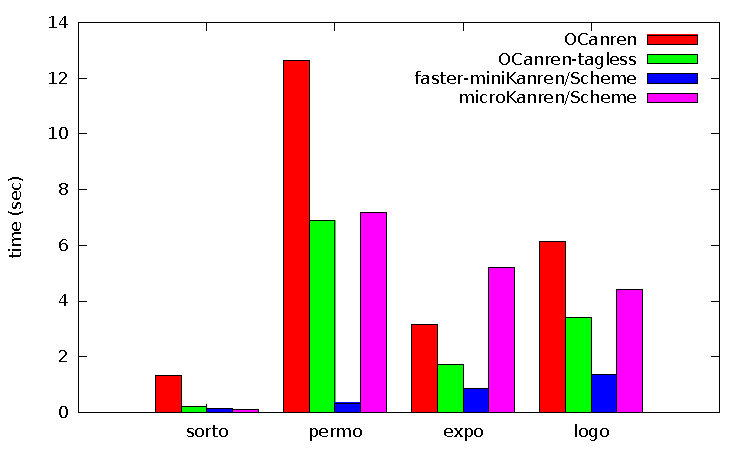
\includegraphics{graph1.pdf}
\caption{The First Set of Benchmarks}
\label{eval:first}
\end{figure}

\begin{figure}[h]
\centering
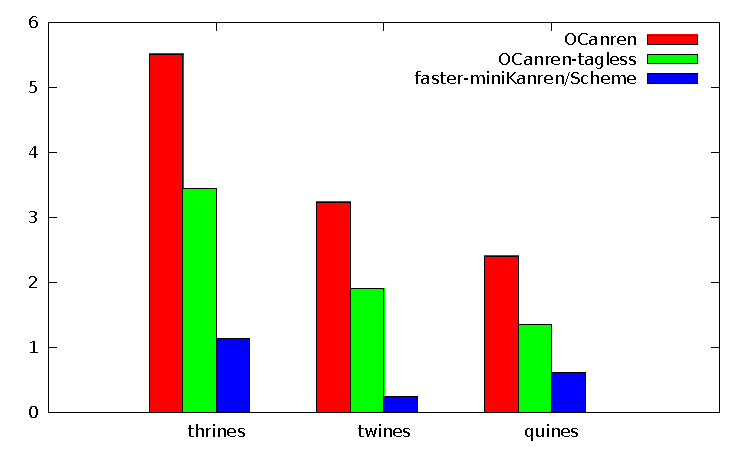
\includegraphics{graph2.pdf}
\caption{The Second Set of Benchmarks}
\label{eval:second}
\end{figure}

\section{Conclusion}

We presented a strongly-typed implementation of \miniKanren for OCaml. Our implementation
passes all tests written for \miniKanren (including those for disequality constraints);
in addition we implemented many interesting relational programs known from
the literature. We claim that our implementation can be used both as a convenient
relational DSL for OCaml and an experimental framework for future research in the area of
relational programming.

%We also want to express our gratitude to William Byrd, who infected us with relational programming,
%and for the extra time he sacrificed as both our tutor and friend.


\begin{thebibliography}{99}
\bibitem{TRS}
Daniel P. Friedman, William E.Byrd, Oleg Kiselyov. The Reasoned Schemer. The MIT
Press, 2005.

\bibitem{MicroKanren}
Jason Hemann, Daniel P. Friedman. $\mu$Kanren: A Minimal Core for Relational Programming //
Proceedings of the 2013 Workshop on Scheme and Functional Programming (Scheme '13).

%\bibitem{alphaKanren}
%William E. Byrd, Daniel P. Friedman. alphaKanren: A Fresh Name in Nominal Logic Programming //
%Proceedings of the 2007 Workshop on Scheme and Functional Programming (Scheme '07).

\bibitem{CKanren}
Claire E. Alvis, Jeremiah J. Willcock, Kyle M. Carter, William E. Byrd, Daniel P. Friedman.
cKanren: miniKanren with Constraints //
Proceedings of the 2011 Workshop on Scheme and Functional Programming (Scheme '11).

\bibitem{Untagged}
William E. Byrd, Eric Holk, Daniel P. Friedman.
miniKanren, Live and Untagged: Quine Generation via Relational Interpreters (Programming Pearl) //
Proceedings of the 2012 Workshop on Scheme and Functional Programming (Scheme '12).

%\bibitem{Kumar}
%Ramana Kumar. Mechanising Aspects of miniKanren in HOL. Bachelor Thesis, The Australian National University, 2010.

\bibitem{Unification}
Franz Baader, Wayne Snyder. Unification theory. In John Alan Robinson and Andrei Voronkov, editors,
Handbook of Automated Reasoning. Elsevier and MIT Press, 2001.

%\bibitem{UnificationRevisited}
%J.-L. Lassez, M.J. Maher, K. Marriott. Unification Revisited // Foundations of Deductive Databases and Logic Programming, 
%Morgan Kaufmann Publishers Inc., 1988.

%\bibitem{Lambda}
%Henk Barendregt. Lambda Calculi with Types, Handbook of Logic in Computer Science (Vol.~2), 1992.

\bibitem{WillThesis}
William E. Byrd. Relational Programming in miniKanren: Techniques, Applications, and Implementations. PhD Thesis,
Indiana University, Bloomington, IN, September 30, 2009.

\bibitem{OCanren}
Dmitry Kosarev, Dmitry Boulytchev. Typed Embedding of a Relational Language in OCaml // International Workshop on ML, 2016.

\bibitem{RelConversion}
Petr Lozov, Andrei Vyatkin, Dmitry Boulytchev. Typed Relational Conversion // International Symposium on Trends in Functional
Programming, 2017.

%\bibitem{Types}
%Benjamin Pierce. Types and Programming Languages. MIT Press, 2002.

%\bibitem{Felleisen}
%Andrew Wright, Matthias Felleisen. A Syntactic Approach to Type Soundness // Information and Computation, Vol.~115, No.~1, 1994.

%\bibitem{cardelli}
%Luca Cardelli, Peter Wegner. On Understanding Types, Data Abstraction, and Polymorphism // ACM Computing Surveys, Vol.~17, No.~4, 1985.

\bibitem{unified}
William E. Byrd, Michael Ballantyne, Gregory Rosenblatt, Matthew Might. A Unified Approach to Solving Seven Programming Problems // 
Proceedings of the International Conference on Functional Programming, 2017.

%\bibitem{WillOnHM}
%William E. Byrd. Personal communications.

\bibitem{Guided}
Cameron Swords, Daniel P. Friedman. rKanren: Guided Search in miniKanren //
Proceedings of the 2013 Workshop on Scheme and Functional Programming (Scheme '13). 

\bibitem{AlphaKanren}
William E. Byrd, Daniel P. Friedman. alphaKanren: A Fresh Name in Nominal Logic Programming //
Proceedings of the 2007 Workshop on Scheme and Functional Programming (Scheme '07).

\bibitem{2016}
Jason Hemann, Daniel P. Friedman, William E. Byrd, Matthew Might.
A Small Embedding of Logic Programming with a Simple Complete Search //
Proceedings of the 12th Symposium on Dynamic Languages (DLS 2016).

\bibitem{CKanren1}
Jason Hemann, Daniel P. Friedman. A Framework for Extending microKanren with Constraints //
Proceedings of the 2015 Workshop on Scheme and Functional Programming (Scheme '15).

\bibitem{Search}
Oleg Kiselyov, Chung-chieh Shan, Daniel P. Friedman, Amr Sabry. Backtracking, Interleaving, and Terminating Monad Transformers (functional pearl) //
Proceedings of the 10th ACM SIGPLAN International Conference on Functional Programming (ICFP '05).

\bibitem{KiselyovArithmetic}
Oleg Kiselyov, William E. Byrd, Daniel P. Friedman, Chung-chieh Shan.
Pure, declarative, and constructive arithmetic relations (declarative pearl) //
Proceedings of the 9th International Symposium on Functional and Logic Programming, 2008.

\end{thebibliography}

\clearpage
\appendix
\section{Appendix}
\label{appendix}

In this appendix we present a proof of partial semantic correctness of relational conversion, or, to be precise, 
a number of observations, definitions, and claims, which, we believe, are sufficient to reconstruct
the complete proof. 

We remind, that our goal is to prove the following statement:

\begin{theorem} 
\normalfont For arbitrary functional program $p$ of a ground type $t$, arbitrary value $v$, and
arbitrary variable $x$

$$
\begin{array}{c}
p\leadsto^f v \Rightarrow \lstinline|fresh ($x$) ($\sembr{p}^c x$)| \leadsto^r (\theta, \emptyset)\\
\mbox{and}\\
\theta(\mathfrak{s})=v
\end{array}
$$

\noindent where $\mathfrak{s}$ is a semantic variable, associated with
$x$ on the first step of the relational evaluation.
\end{theorem}
  
We first comment on the empty set as the set of negative substitutions. A disequality constraint can
come only from a polymorphic equality, which is applied when both its operands are reduced to
values. In the relational counterpart, being run in a forward direction, this corresponds to the evaluation of disequality constraints for
closed terms only, which, in turn, means, that they will immediately succeed or fail. Both cases
add nothing to the set of negative substitutions, which is initially empty. 

Next, we cannot prove the theorem, using an induction by a derivation length, since in the case of
application, for example, the type of the term in the head position is not ground. This 
obstacle could be lifted, if we could prove the following generalization:

$$
p\leadsto^f f \Rightarrow \sembr{p}^c\leadsto^r\sembr{f}^c
$$ 

\noindent for arbitrary $p$ of any type. This claim, however, turned out to be false~--- a term
\lstinline|C ((fun x.x) A)| can be taken as an example.  

The origin of the problem is that we \emph{functionalize} the constructors, \lstinline|match|, and
equality expressions, and, hence, change the order of reductions in the relational counterpart in 
comparison with the original functional program. Thus, we need to take this change into account.

First, we develop a modified functional semantics, which corresponds better to the reduction
order in the relational case. We call this semantics \emph{deferred}, as it defers the evaluation
of constructors, \lstinline|match|, and equality expressions. This semantics can be acquired in
two steps: first, we consider a reduced version of the original functional semantics, in which
we treat arbitrary constructor, \lstinline|match|, and equality expressions as values. Then, the
deferred semantics is just an iterative application of the reduced version to the arguments 
of these new values (arguments of constructors or equality operator, or scrutinees of \lstinline|match| 
expressions).

Next, we claim, that if a term of some ground type is reduced to some value by the original semantics,
then it as well is reduced to the same value by the deferred one. This claim is based on the following
observations:

\begin{itemize}
\item progress and type preservation properties for both semantics (which can be proven in a standard
way);
\item Church-Rosser property for lambda-calculus;
\item the fact, that the reduced semantics applies a proper subset of rules of the original one.
\end{itemize}

Now, we are going to prove the theorem by a simulation between the deferred semantics for the original program
and the relational one for the relationally converted. Before that, we formulate the number of lemmas and 
definitions.

\begin{lemma}
\label{stack_split}
\normalfont Let us separate all the contexts into two disjoint kinds: 

\begin{itemize}
\item functional

$$
C_f = \Box\;e\mid v\;\Box\mid\lstinline|let $x$ = $\Box$ in $e$|
$$

\item ground

$$
C_g = \lstinline|match $\;\Box\;$ with $\{p_i$->$e_i\}$|\mid C^n(\bar{v},\Box,\bar{e})\mid\Box\lstinline|=e|\mid\lstinline|v=|\Box
$$

Let $\left<{\mathcal S},\,e\right>$ be an arbitrary state in a derivation sequence w.r.t. the deferred
semantics. Then $\mathcal S=C_f^*C_g^*$.
\end{itemize}

In other words, during the evaluation w.r.t. the deferred semantics, the stack of contexts is separated into the two
(possibly empty) segments: all ground contexts reside below all functional. The proof is by the induction on the
length of derivation sequence.
\end{lemma}

\begin{definition}
\normalfont
We as well separate all terms of the source language into the two disjoint kinds:

\begin{itemize}
\item functional

$$
e_1\,e_2\mid \lambda x.e \mid \mu f.\lambda x.e \mid \lstinline|let $x$ = $e_1$ in $e_2$| \mid \lstinline|let rec $f$ = $\lambda x.e_1$ in $e_2$|
$$

\item ground

$$
e_1 = e_2 \mid \lstinline|match $e$ with {$p_i$ -> $e_i$ }| \mid \lstinline|C$^k$ ($e_1\dots e_k$)|
$$

\end{itemize}

\end{definition}

\begin{definition}
\normalfont Augmented conversion of a term w.r.t. to a substitution $\sembr{\bullet}_\theta$ is defined as follows: 

$$
\begin{array}{rcl}
\sembr{p}_\theta&=&\sembr{p}^c\\
\sembr{v}_\theta&=&(\lambda x.x\equiv\mathfrak{s}),\,\mbox{if}\;\;\theta(\mathfrak s)=v
\end{array}
$$

Here $\theta$ is a substitution, $p$~--- arbitrary functional term, $v$~--- arbitrary value of a
ground type in the sense of the original semantics (i.e. the composition of constructors). Note, the
cases in this definition are not disjoint, and in the second case there can be more, than one
variable with the requested property, so augmented conversion defines a set of relational terms.
\end{definition}

\begin{lemma}
\label{substitution}
\normalfont Let $f$, $e$ be two arbitrary terms of the source language, $\theta$~--- arbitrary
substitution. Then

$$
\sembr{f[x\gets e]}_\theta=\sembr{f}_\theta[x\gets\sembr{e}_\theta]
$$

The equality here is understood in a set-theoretic sense. The proof is by structural 
induction.
\end{lemma}

\begin{definition}
\normalfont For arbitrary substitution $\theta$ define a conversion of a functional context  
$\sembr{\bullet}_\theta$ as follows:

$$
\begin{array}{rcl}
\sembr{\Box\,e}_\theta&=&\Box\,\sembr{e}_\theta\\
\sembr{v\,\Box}_\theta&=&\sembr{v}_\theta\,\Box\\
\sembr{\lstinline|let $\;x\; = \;\Box\;$ in $\;e$|}_\theta&=&\lstinline|let $\;x\; = \;\Box\;$ in $\;\sembr{e}_\theta$|
\end{array}
$$

Here $e$ is an arbitrary functional term, $v$~--- abstraction. This conversion is an extension of augmented
conversion for functional contexts, hence the same denotation.
\end{definition}

\begin{definition}
\normalfont For arbitrary semantic variables ${\mathfrak s}_1$, ${\mathfrak s}_2$ and arbitrary substitution $\theta$ 
define a conversion of ground context $\sembr{\bullet}^{{\mathfrak s}_1{\mathfrak s}_2}_\theta$ as follows:

$$ 
\begin{array}{rcl}
\sembr{C^k(v_1, \ldots, v_{i-1}, \Box, e_{i+1}, \ldots, e_k)}^{{\mathfrak s}_1{\mathfrak s}_2}_\theta&=&\Box \; \wedge \\
       & & (\sembr{e_{i+1}}_\theta \; {\mathfrak s}^\prime_{i+1}) \; \wedge \\
       & & \ldots  \\
       & & (\sembr{e_k}_\theta \; {\mathfrak s}^\prime_k) \; \wedge \\
       & & ({\mathfrak s}_2 \equiv\; \uparrow C^k({\mathfrak s}^\prime_1, \ldots, {\mathfrak s}^\prime_{i-1}, {\mathfrak s}_1, {\mathfrak s}^\prime_{i+1}, \ldots, {\mathfrak s}_k)),\,\mbox{if}\;\theta({\mathfrak s}^\prime_j)=v_j,\,j<i
\end{array}
$$

$$
\begin{array}{rcl}
\sembr{\Box = e}^{{\mathfrak s}_1{\mathfrak s}_2}_\theta&=&\Box\, \wedge \\
 & & (\sembr{e}_\theta\; {\mathfrak s}^\prime) \wedge \\
 & & ((({\mathfrak s}_1 \equiv {\mathfrak s}^\prime) \wedge ({\mathfrak s}_2 \equiv \lstinline|^true|))\, \vee \\ 
 & & (({\mathfrak s}_1 \not \equiv {\mathfrak s}^\prime) \wedge ({\mathfrak s}_2 \equiv \lstinline|^false|))) 
\end{array}
$$

$$
\begin{array}{rcl}
\sembr{v = \Box}^{{\mathfrak s}_1{\mathfrak s}_2}_\theta&=&\Box\,\wedge \\
 & & ((({\mathfrak s}^\prime \equiv {\mathfrak s}_1) \wedge ({\mathfrak s}_2 \equiv \lstinline|^true|))\, \vee \\ 
 & & (({\mathfrak s}^\prime \not \equiv {\mathfrak s}_1) \wedge ({\mathfrak s}_2 \equiv \lstinline|^false|))),\,\mbox{if}\;\theta({\mathfrak s})=v 
\end{array}
$$

$$
\begin{array}{rcl}
\sembr{\lstinline|match $\;\Box\;$ with \{$C^{n_i}_i$($y^i_1$, ..., $y^i_{n_i}$) -> $\;e_i$\}|}^{{\mathfrak s}_1{\mathfrak s}_2}_\theta&=&\Box \; \wedge \bigvee_i\\
& &(\lstinline|fresh ($s^i_1 \ldots s^i_{n_i}$)| \\
& &\qquad({\mathfrak s}_1 \equiv \;\uparrow C_i^{n_i}(s^i_1, \ldots, s^i_{n_i})) \\
& &\qquad(\lambda y^i_1. \ldots \lambda  y^i_{n_i}. \sembr{e_i}_\theta) \; (\equiv s^i_1) \ldots (\equiv s^i_{n_i})\;{\mathfrak s}_2)
\end{array}
$$

Here we assume ${\mathfrak s}^\prime$ and ${\mathfrak s}^\prime_i$ to be arbitrary semantic variables, $v_i$~--- arbitrary values w.r.t. the original 
functional semantics, $e_i$~--- arbitrary terms of the source language. We also claim, that $\theta$ is
undefined for all mentioned semantic variables, unless the opposite is specified explicitly.

\end{definition}

\begin{definition}
\normalfont For arbitrary substitution $\theta$, arbitrary semantic variable ${\mathfrak s}_m$ and a functional 
term $e$ define a conversion of a stack $\sembr{\bullet}^{e,{\mathfrak s}_m}_\theta$ as follows:

$$
\def\arraystretch{1.5}
\sembr{f_n\dots f_1g_m\dots g_1}^{e,{\mathfrak s}_m}_\theta=\left\{
\begin{array}{lcl}
\sembr{g_m}^{{\mathfrak s}_m{\mathfrak s}_{m-1}}_\theta\dots\sembr{g_1}^{{\mathfrak s}_1{\mathfrak s}_0}_\theta&,&n=0\;\;\mbox{and $e$~--- ground}\\
\sembr{f_n}_\theta\dots\sembr{f_1}_\theta(\Box\,{\mathfrak s}_m)\sembr{g_m}^{{\mathfrak s}_m{\mathfrak s}_{m-1}}_\theta\dots\sembr{g_1}^{{\mathfrak s}_1{\mathfrak s}_0}_\theta&,&\mbox{otherwise}
\end{array}
\right.
$$

Here ${\mathfrak s}_0\dots {\mathfrak s}_{m-1}$ designate arbitrary distinct semantic variables.
\end{definition}

\begin{definition}
\normalfont For arbitrary substitution $\theta$ and arbitrary semantic variable ${\mathfrak s}_m$ define a simulation
conversion $\sembr{\bullet}^{{\mathfrak s}_m}_\theta$ of the source language term as follows:

$$
\begin{array}{rcl}
\sembr{e_1 = e_2}^{{\mathfrak s}_m}_\theta&=& (\sembr{e_1}_\theta\; {\mathfrak s}^\prime_1) \wedge \\
                           & & (\sembr{e_2}_\theta\; {\mathfrak s}^\prime_2) \wedge \\
                           & & ((({\mathfrak s}^\prime_1 \equiv {\mathfrak s}^\prime_2) \wedge ({\mathfrak s}_m \equiv \lstinline|^true|))\, \vee \\ 
                           & & (({\mathfrak s}^\prime_1 \not \equiv {\mathfrak s}^\prime_2) \wedge ({\mathfrak s}_m \equiv \lstinline|^false|)))
\end{array}
$$

$$
\begin{array}{rcl}
\sembr{v = e}^{{\mathfrak s}_m}_\theta&=& (\sembr{e}_\theta\; {\mathfrak s}^\prime_2) \wedge \\
                        & & ((({\mathfrak s}^\prime_1 \equiv {\mathfrak s}^\prime_2) \wedge ({\mathfrak s}_m \equiv \lstinline|^true|))\, \vee \\ 
                        & & (({\mathfrak s}^\prime_1 \not \equiv {\mathfrak s}^\prime_2) \wedge ({\mathfrak s}_m \equiv \lstinline|^false|))),\,\mbox{if}\;\theta({\mathfrak s}^\prime_1)=v
\end{array}
$$

$$
\begin{array}{rcl}
\sembr{v_1 = v_2}^{{\mathfrak s}_m}_\theta&=& ((({\mathfrak s}^\prime_1 \equiv {\mathfrak s}^\prime_2) \wedge ({\mathfrak s}_m \equiv \lstinline|^true|))\, \vee \\ 
                           & & (({\mathfrak s}^\prime_1 \not \equiv {\mathfrak s}^\prime_2) \wedge ({\mathfrak s}_m \equiv \lstinline|^false|))),\,\mbox{if}\;\theta({\mathfrak s}^\prime_j)=v_j
\end{array}
$$

$$ 
\begin{array}{rcl}
\sembr{C^k(v_1, \ldots, v_{i-1}, e_i, \ldots, e_k)}^{{\mathfrak s}_m}_\theta&=&(\sembr{e_i}_\theta \; {\mathfrak s}^\prime_i) \; \wedge \\
       & & \ldots  \\
       & & (\sembr{e_k}_\theta \; {\mathfrak s}^\prime_k) \; \wedge \\
       & & ({\mathfrak s}_m \equiv\; \uparrow C^k({\mathfrak s}^\prime_1, \ldots, {\mathfrak s}^\prime_k)),\,\mbox{if}\;\theta({\mathfrak s}^\prime_j)=v_j,\,j<i
\end{array}
$$

$$ 
\sembr{C^k(v_1, \ldots, v_k)}^{{\mathfrak s}_m}_\theta = ({\mathfrak s}_m \equiv\; \uparrow C^k({\mathfrak s}^\prime_1, \ldots, {\mathfrak s}^\prime_k)),\,\mbox{if}\;\theta({\mathfrak s}^\prime_j)=v_j
$$

$$ 
\sembr{C^k(v_1, \ldots, v_k)}^{{\mathfrak s}_m}_\theta = ({\mathfrak s}_m \equiv\; {\mathfrak s}^\prime),\;\mbox{if}\;\theta({\mathfrak s}^\prime)=C^k(v_1, \ldots, v_k)
$$

$$
\begin{array}{rcl}
\sembr{\lstinline|match $\;e\;$ with \{$C^{n_i}_i$($y^i_1$, ..., $y^i_{n_i}$) -> $\;e_i$\}|}^{{\mathfrak s}_m}_\theta&=&\sembr{e}_\theta\;{\mathfrak s}^\prime\;\wedge\;\bigvee_i\\
& &(\lstinline|fresh ($s^i_1 \ldots s^i_{n_i}$)| \\
& &\qquad({\mathfrak s}^\prime \equiv \;\uparrow C_i^{n_i}(s^i_1, \ldots, s^i_{n_i})) \\
& &\qquad(\lambda y^i_1. \ldots \lambda  y^i_{n_i}. \sembr{e_i}_\theta) \; (\equiv s^i_1) \ldots (\equiv s^i_{n_i})\;{\mathfrak s}_m)
\end{array}
$$

$$
\begin{array}{rcl}
\sembr{\lstinline|match $\;v\;$ with \{$C^{n_i}_i$($y^i_1$, ..., $y^i_{n_i}$) -> $\;e_i$\}|}^{{\mathfrak s}_m}_\theta&=&\bigvee_i\\
& &(\lstinline|fresh ($s^i_1 \ldots s^i_{n_i}$)| \\
& &\qquad({\mathfrak s}^\prime \equiv \;\uparrow C_i^{n_i}(s^i_1, \ldots, s^i_{n_i})) \\
& &\qquad(\lambda y^i_1. \ldots \lambda  y^i_{n_i}. \sembr{e_i}_\theta) \; (\equiv s^i_1) \ldots (\equiv s^i_{n_i})\;{\mathfrak s}_m),\,\mbox{if}\;\theta({\mathfrak s}^\prime)=v
\end{array}
$$

Here all ${\mathfrak s}^\prime$ and ${\mathfrak s}^\prime_i$ designate arbitrary semantic variables, $e$~--- arbitrary term, $v$~--- arbitrary value w.r.t. the
original semantics. We also claim, that $\theta$ is undefined for all mentioned semantic variables, unless the opposite is specified explicitly.
\end{definition}

\begin{definition}
\normalfont Let 
\begin{itemize}
\item \mbox{$\left<\mathcal S,\,e\right>$}~--- a state w.r.t. the deferred semantics;
\item \mbox{$\left<\Sigma, \hat{\mathcal S}, \hat{e}, (\theta, \emptyset)\right>$}~--- a state w.r.t. the
relational semantics.
\end{itemize} 

We say, that these states are connected, if there exists a semantic variable $q_m$, such, that:\vspace{1mm}

\begin{enumerate}
\item \mbox{$\hat{\mathcal S}\in\sembr{\mathcal S}^{e,{\mathfrak s}_m}_\theta$}\vspace{1mm}
\item \mbox{$\hat{e}\in\left\{
                          \begin{array}{lcl}
                            \sembr{e}^{{\mathfrak s}_m}_\theta&,&e\mbox{~--- ground and }\mathcal S\mbox{ does not contain functional contexts}\\[1mm]
                            \sembr{e}_\theta&,&\mbox{otherwise}
                          \end{array}
                       \right.
            $} 
\item $\Sigma$ contains all semantic variables from $\hat{e}$, $\hat{\mathcal S}$, and $\theta$.
\end{enumerate}

\end{definition}

\begin{lemma}
\label{constructor}
\normalfont Let $v=\lstinline|C$^k$($v_1$,...,$v_k$)|$ be a value. Then
for arbitrary $\Sigma$, $\mathcal S$, $\theta$, $\hat{v}\in \sembr{v}_\theta$, and 
semantic variable ${\mathfrak s}$, such, that ${\mathfrak s}\not\in dom(\theta)$ either

$$
\left<\Sigma,\,\mathcal S, (\hat{v}\,{\mathfrak s}),\, (\theta,\,\emptyset)\right>\leadsto^*\left<\Sigma^\prime,\,\mathcal S,\,{\mathfrak s}\equiv\lstinline|C$^k$(${\mathfrak s}^\prime_1$,...,${\mathfrak s}^\prime_k$)|,\,(\theta^\prime,\,\emptyset)\right>\;\mbox{and}\;\theta^\prime({\mathfrak s}^\prime_i)=v_i
$$

or

$$
\left<\Sigma,\,\mathcal S, (\hat{v}\,{\mathfrak s}),\, (\theta,\,\emptyset)\right>\leadsto\left<\Sigma,\,\mathcal S,\,{\mathfrak s}\equiv {\mathfrak s}^\prime,\,(\theta,\,\emptyset)\right>\;\mbox{and}\;\theta({\mathfrak s}^\prime)=v
$$
 
The proof is by induction on the height of $v$.
\end{lemma}

\begin{lemma}
\label{evaluation_lemma}
\normalfont Let $s=\left<\mathcal S=g_m\dots g_1,\,e\right>$ be a state w.r.t. the deferred semantics, 
$g_i$~--- ground contexts, $e$~--- expression of a ground type, $\theta$~--- some substitution,
${\mathfrak s}_m$~--- some semantic variable, \mbox{$\hat{\mathcal{S}}\in\sembr{\mathcal S}^{e,\,{\mathfrak s}_m}_\theta$}, 
\mbox{$\hat{e} \in \sembr{e}_\theta$}. Then there is a sequence of steps w.r.t. the relational
semantics, such, that

$$
\left<\Sigma, \hat{\mathcal S}, (\hat{e} \, {\mathfrak s}_m), (\theta,\,\emptyset) \right>\leadsto^*\hat{s}
$$

\noindent and $s$ and $\hat{s}$ are connected. Here we assume $\Sigma$ to contain all semantic variables from
$\hat{\mathcal S}$ and $\theta$. The proof is by case analysis on $e$, using Lemma~\ref{constructor}.
\end{lemma}

\begin{lemma} 
\label{connection}
\normalfont Let \mbox{$s_1 \to s_2$}~--- a single evaluation step w.r.t. the deferred semantics,
$\hat{s_1}$~--- a state of the relational semantics, such, that $s_1$ and $\hat{s_1}$ are connected. Then
there exists a sequence of steps in the relational semantics \mbox{$\hat{s_1}\leadsto^*\hat{s_2}$}, such, 
that $s_2$ and $\hat{s_2}$ are connected. The proof is by case analysis and definition of connection
relation, using Lemmas~\ref{substitution},~\ref{constructor},~\ref{evaluation_lemma}. 
\end{lemma}

\begin{lemma}
\label{prefix}
\normalfont Let $s_0=\left<\emptyset,\,\epsilon,\,\lstinline|fresh ($x$) $(\sembr{e}^c\;x)$|,\,\iota\right>$ be an
initial state of evaluation w.r.t. the relational semantics. Then there is a sequence of steps
\mbox{$s_0\leadsto^*\hat{s}$}, such, that \mbox{$\left<\epsilon,\,e\right>$} (an initial state of
evaluation of $e$ w.r.t. the deferred semantics) and $\hat{s}$ are connected. Immediately follows from
Lemma~\ref{evaluation_lemma}.
\end{lemma}

Now we can prove the partial correctness theorem. Let us have a term $e$ of a ground type in the source language, which
reduces to a value $v=\lstinline|C$^k$($v_1$,...,$v_k$)|$ w.r.t. the original call-by-value semantics. Then it reduces to the same value w.r.t. the
deferred semantics: 

$$
\left<\epsilon,\,e\right>\to^*\left<\epsilon,\,v\right>
$$

By Lemma~\ref{prefix} 

$$
\left<\emptyset,\,\epsilon,\lstinline|fresh ($x$) $(\sembr{e}^c\;x)$|,\iota\right>\leadsto^*\hat{s}
$$

\noindent where \mbox{$\left<\epsilon,\,e\right>$} and $\hat{s}$ are connected. By Lemma~\ref{connection}, there is
a state $\hat{s^\prime}$ w.r.t. the relational semantics, such, that

$$
\hat{s}\leadsto^*\hat{s^\prime}
$$

\noindent and \mbox{$\left<\epsilon,\,v\right>$} and $\hat{s^\prime}$ are connected. By the definition of
the connection relation, $\hat{s^\prime}$ has one of the following forms:

$$
\left<\Sigma,\,\epsilon,\,{\mathfrak s}_0\equiv\lstinline|C$^k$(${\mathfrak s}^\prime_1$,...,${\mathfrak s}^\prime_k$)|,\,(\theta,\,\emptyset)\right>,\,\theta({\mathfrak s}^\prime_i)=v_i
$$

\noindent or

$$
\left<\Sigma,\,\epsilon,\,{\mathfrak s}_0\equiv {\mathfrak s}^\prime,\,(\theta,\,\emptyset)\right>,\,\theta({\mathfrak s}^\prime)=v
$$

\noindent where ${\mathfrak s}_0$ is the first semantic variable, added to $\Sigma$, and \mbox{${\mathfrak s}_0\not\in dom(\theta)$}. In
both cases, we can make the one last step in the relational semantics, which completes the proof. 


\end{document}
